% !TeX program = xelatex
% 编译：cd documents/fix_docs && xelatex -interaction=nonstopmode fix-20261030.tex（跑两遍）
% 修复前 = main，修复后 = fix-20261030。例子取自 2015--2021 年样本（2012--2014 年作历史），
% 1972 年前的例子取自 1968--1975 年样本；两边用同一份原始数据。
\documentclass[UTF8,fontset=fandol,aspectratio=169,10pt,t]{ctexbeamer}
\usepackage{booktabs,graphicx,array,colortbl}
\setmainfont{texgyretermes-regular.otf}[BoldFont=texgyretermes-bold.otf,ItalicFont=texgyretermes-italic.otf]
\setmonofont{lmmono10-regular.otf}

\usetheme{default}
\usecolortheme{seahorse}
\setbeamertemplate{navigation symbols}{}
\setbeamertemplate{footline}{\hfill\scriptsize\insertframenumber/\inserttotalframenumber\hspace{6pt}\vspace{4pt}}
\setbeamerfont{frametitle}{series=\bfseries,size=\large}
\setbeamercolor{frametitle}{fg=black!85,bg=blue!8}
\setbeamertemplate{itemize items}{\textbullet}
\setbeamercolor{item}{fg=black!70}
\setlength{\leftmargini}{1.1em}

% 红字 = 修复后变了的值
\newcommand{\chg}[1]{\textcolor{red!80!black}{#1}}
\newcommand{\kong}{空}
\newcommand{\code}[1]{\texttt{#1}}
\newcommand{\lab}[1]{\textbf{#1}\quad}
\newcommand{\tsize}{\small}
\newcommand{\src}[1]{{\footnotesize\color{black!60}#1}}
\setlength{\aboverulesep}{0.4ex}\setlength{\belowrulesep}{0.4ex}
\renewcommand{\arraystretch}{1.12}

\title{20261030 指标修复说明}
\subtitle{修复前 = \code{main}，修复后 = \code{fix-20261030}}
\date{2026 年 11 月}

\begin{document}

\begin{frame}
\titlepage
\end{frame}

\begin{frame}{先说几句}
\begin{itemize}
\item 每个指标两页：第一页讲它是什么、基准（HXZ 2020、GHZ 2017、JKP 2023、Chen--Zimmermann）怎么做、我们原来哪里不对；第二页讲改了什么，再放一张修复前后的对比表。
\item 表里的列名就是最终文件 \code{chars\_raw\_no\_impute.parquet} 里的列名。\code{date} 是最终文件里的 \code{date}，也就是收益所在的月份，指标在它上个月末算好。
\item \chg{红字}是修复后变了的值，“\kong”是缺失。只有 \code{sgrvol} 一组用的是季度中间文件 \code{chars\_q\_accounting.parquet}，因为最终文件里没有它。
\item 例子来自 2015--2021 年的样本（2012--2014 年作历史），1972 年以前的例子来自 1968--1975 年的样本。两边用的是同一份原始数据。
\end{itemize}
\end{frame}

%======================================================================
\begin{frame}{sue：标准化未预期盈利}
\begin{itemize}
\item \lab{指标}最近一个季度的每股收益相对去年同季的变化，除以过去 8 个季度这种变化的标准差。
\item \lab{基准做法}HXZ A.1.1。1972 年起，季度盈利要等公告日 \code{rdq} 过了才能用；1972 年以前没有 \code{rdq}，季末后 4 个月才能用。季末离当前超过 6 个月的季度不再用。过去 8 个季度的变化至少要有 6 个。
\item \lab{我们的问题}原来只看季末 \code{datadate} 过没过，季度还没公告就拿来用了：2015--2021 年差不多一半的月份用到了尚未公告的季度。过期窗口是 12 个月。历史 EPS 是“往前数 $k$ 行”，中间缺一个季度就整体错位。
\end{itemize}
\end{frame}

\begin{frame}{sue：修正与前后对比}
\lab{修正}改成 \code{rdq} 不晚于月末才能用（1972 年前用季末 + 4 个月），窗口改为 6 个月；历史 EPS 按同一 gvkey、往前正好 $3k$ 个月的季度去找。\par\medskip
\begin{minipage}[t]{0.46\linewidth}
\src{permno 10028，2018Q4 到 2019-04-12 才公告。修复前 1 月起就在用它。}\par\smallskip
{\tsize
\begin{tabular}{l rr}
\toprule
date & sue（前） & sue（后） \\
\midrule
2019-03-31 & $-0.158$ & \chg{$-0.559$} \\
2019-04-30 & $-0.158$ & \chg{$-0.559$} \\
2019-05-31 & $0.000$ & \chg{$-0.158$} \\
2019-06-30 & $0.000$ & $0.000$ \\
\bottomrule
\end{tabular}}
\end{minipage}\hfill
\begin{minipage}[t]{0.46\linewidth}
\src{1972 年以前，permno 44396。修复前季度结束当月就用了。}\par\smallskip
{\tsize
\begin{tabular}{l rr}
\toprule
月份 & sue（前） & sue（后） \\
\midrule
1970-12 & 5.752 & \chg{0.604} \\
1971-01 & 5.752 & \chg{2.831} \\
1971-04 & $-0.347$ & \chg{5.752} \\
\bottomrule
\end{tabular}}
\par\medskip
\end{minipage}
\src{1972 年前的样本只跑到 \code{sue.parquet}，按形成月份列出。}
\end{frame}

%======================================================================
\begin{frame}{abr：盈余公告前后的累计超额收益}
\begin{itemize}
\item \lab{指标}公告日前 2 个交易日到后 1 个交易日，个股日收益减市场日收益的累计。
\item \lab{基准做法}HXZ A.1.2。公告日必须晚于季末；季末离当前不超过 6 个月。
\item \lab{我们的问题}不检查 \code{rdq} 是否晚于季末。过期窗口 12 个月，过期的 abr 一直挂着（约 4\% 的月份）。同一天公告好几个季度时，日收益被加了好几遍（161 个公告）。先删掉缺失收益再数交易日，窗口会滑到别的日子（347 个值）。
\end{itemize}
\end{frame}

\begin{frame}{abr：修正与前后对比}
\lab{修正}要求 \code{rdq} 晚于 \code{datadate}；窗口改为 6 个月；每个（permno，公告日）只留一个事件；先数交易日再求和。市场收益仍用 \code{mktrf + rf}。\par\medskip
\src{permno 92805，季末 2015-03-31，拖到 2015-08-11 才公告，之后 Compustat 里再没有新季度。修复前这个 abr 一直用到 2016 年 4 月。}\par\smallskip
{\tsize
\begin{tabular}{l rr}
\toprule
date & abr（前） & abr（后） \\
\midrule
2015-10-31 & 0.0187 & 0.0187 \\
2015-11-30 & 0.0187 & \chg{\kong} \\
2016-01-31 & 0.0187 & \chg{\kong} \\
2016-04-30 & 0.0187 & \chg{\kong} \\
\bottomrule
\end{tabular}}
\end{frame}

%======================================================================
\begin{frame}{re：分析师盈利预测修正}
\begin{itemize}
\item \lab{指标}过去 6 个月当年财年（FY1）一致预测的月度变化，除以上月股价，再加总。
\item \lab{基准做法}HXZ A.1.3（式 A2）。只用 FY1；月度修正 $=(f_t-f_{t-1})/p_{t-1}$；对最近 6 个月的修正求和，至少要有 4 个。财年结束到实际值公布之间，FY1 仍然是刚结束的那个财年。
\item \lab{我们的问题}FY2 混进来了。\code{unique()} 打乱顺序后再 \code{shift}，滞后错位。用的是 $t-6$ 到 $t-1$，晚了一个月，而且取的是平均不是求和。下载条件 \code{fpedats >= statpers} 把财年结束后的 FY1 全删了。CRSP 累计调整因子为 0 时除法直接报错。
\end{itemize}
\end{frame}

\begin{frame}{re：修正与前后对比}
\lab{修正}只保留 FPI = 1。月度修正要求上一条预测正好是上个月。滞后按日历月取，和当月合起来有 4 个以上就求和。下载去掉 \code{fpedats >= statpers}，re 的覆盖多了 84\%。调整因子为 0 当作缺失。\par\medskip
\src{IBM（permno 12490），FY2017，单位 $10^{-4}$。IBM 1 月换财年，1 月没有修正；修复前 4、5 月拿到的其实是 FY2018 的预测。}\par\smallskip
{\tsize
\begin{tabular}{l rr}
\toprule
date & re（前） & re（后） \\
\midrule
2017-04-30 & $-1.82$ & \chg{0.54} \\
2017-05-31 & $0.54$ & \chg{$-3.60$} \\
2017-06-30 & $-1.90$ & \chg{$-4.25$} \\
2017-07-31 & $-2.49$ & \chg{$-4.25$} \\
\bottomrule
\end{tabular}}
\end{frame}

%======================================================================
\begin{frame}{财务滞后：agr 以及所有要用上期值的指标}
\begin{itemize}
\item \lab{指标}agr 是总资产同比增长。同样的滞后用在 ni、chcsho、cinvest、roavol、ttm4 等大约 100 处。
\item \lab{基准做法}JKP。上期值要来自同一家公司（gvkey），并且正好早 $k$ 期：年度差 12 个月，季度差 3 个月。
\item \lab{我们的问题}\code{shift(k).over('permno')} 是往前数行。permno 换了 gvkey，就拿到前一家公司的数；中间缺一期，就拿到更早的那期。
\end{itemize}
\end{frame}

\begin{frame}{财务滞后：修正与前后对比}
\lab{修正}\code{functions.py} 加了 \code{lag(列, k, months)}：同 permno、同 gvkey、日期正好差 $k$ 期（容差不到一期，财年月份变更也能对上）。99.7\% 的值没变，约 1\% 置空。1968--1975 年的季度覆盖反而多了，因为 main 把年度和季度混排后行距本来就不对。\par\medskip
\src{permno 10253，2013 年 7 月 gvkey 从 012200 换成 018290。新公司一年前没有资产数据，修复前的 agr 拿的是老公司 2012 年的总资产。}\par\smallskip
{\tsize
\begin{tabular}{l l rr}
\toprule
date & gvkey & agr（前） & agr（后） \\
\midrule
2014-05-31 & 018290 & 3.914 & \chg{\kong} \\
2014-06-30 & 018290 & 3.914 & \chg{\kong} \\
2014-07-31 & 018290 & 3.914 & \chg{\kong} \\
\bottomrule
\end{tabular}}
\end{frame}

%======================================================================
\begin{frame}{ni：股本净发行}
\begin{itemize}
\item \lab{指标}拆股调整后股数的对数同比变化。
\item \lab{基准做法}HXZ A.3.10。$\log(\text{csho}\times\text{ajex})-\log(\text{一年前同值})$；任何一期股数缺失或非正，就缺失。
\item \lab{我们的问题}缺失时 \code{fill\_null(0)}，结果变成 $\log(\text{股数})-0$，也就是股数本身的对数。季度 7.5\%、年度 6.9\% 的 ni 是这种值。
\end{itemize}
\end{frame}

\begin{frame}{ni：修正与前后对比}
\lab{修正}两期股数都为正才算，否则为空。\par\medskip
\src{permno 18100（gvkey 034077），2019Q1 的一年前（2018Q1）没有 cshoq。修复前的 3.446 就是 $\log(31.369)$。}\par\smallskip
{\tsize
\begin{tabular}{l rr}
\toprule
date & ni（前） & ni（后） \\
\midrule
2019-08-31 & 3.446 & \chg{\kong} \\
2019-09-30 & 3.446 & \chg{\kong} \\
2019-10-31 & 3.446 & \chg{\kong} \\
\bottomrule
\end{tabular}}
\end{frame}

%======================================================================
\begin{frame}{roa：季度总资产收益率}
\begin{itemize}
\item \lab{指标}季度净利润 \code{ibq} 除以上季度总资产 \code{atq}。
\item \lab{基准做法}HXZ A.4.3。用最近一次公告（\code{rdq}）的季度盈利，公告日必须晚于季末，季末要在 6 个月以内。其他非盈利类的季度项目仍用季末 + 4 个月。
\item \lab{我们的问题}有一段“尽量用最新 ibq”的代码，把 \code{ibq} 换成下一季度的值，分母 \code{atq\_l1} 却还是本季度的上一季，分子分母差了一个季度。
\end{itemize}
\end{frame}

\begin{frame}{roa：修正与前后对比}
\lab{修正}删掉那段替换。roa 先按季度算 $\text{ibq}_q/\text{atq}_{q-1}$，输出时按每个月最近一次公告取值，季末超过 6 个月不再用（没有 \code{rdq} 时退回季末 + 4 个月）。\par\medskip
\src{permno 10026，2018 年。Q2 于 7 月 30 日公告，Q3 于 11 月 8 日公告。修复前 8 月那行分子是 Q2 的 ibq（26.129），分母却是上一年 Q4 的 atq（865.017），而不是 Q1 的 887.549。}\par\smallskip
{\tsize
\begin{tabular}{l rr l}
\toprule
date & roa（前） & roa（后） & 修复后用的季度 \\
\midrule
2018-08-31 & 0.0302 & \chg{0.0294} & 2018Q2（7 月 30 日公告） \\
2018-11-30 & 0.0294 & 0.0294 & 2018Q2 \\
2018-12-31 & 0.0294 & \chg{0.0256} & 2018Q3（11 月 8 日公告） \\
\bottomrule
\end{tabular}}
\end{frame}

%======================================================================
\begin{frame}{cinvest：企业投资变化}
\begin{itemize}
\item \lab{指标}本季度 \code{ppentq/saleq} 的变化，相对前 3 个季度同样变化的平均值。
\item \lab{基准做法}GHZ。要有本季度和前 4 个季度的数据，不够就置空。
\item \lab{我们的问题}前几期缺失也照算，平均数只用有的那几期。
\end{itemize}
\end{frame}

\begin{frame}{cinvest：修正与前后对比}
\lab{修正}\code{ppentq\_l1} 到 \code{l4} 都有值才算（\code{lag()} 取同一家公司）。4.3\% 的值置空。\par\medskip
\src{permno 14423（gvkey 027046），2016Q1 才开始有 ppentq。2016Q4 那期（2017 年 5--7 月在用）前面只有 3 个季度。}\par\smallskip
{\tsize
\begin{tabular}{l rr}
\toprule
date & cinvest（前） & cinvest（后） \\
\midrule
2017-05-31 & 1.5 & \chg{\kong} \\
2017-06-30 & 1.5 & \chg{\kong} \\
2017-08-31 & 0.4 & 0.4 \\
\bottomrule
\end{tabular}}
\end{frame}

%======================================================================
\begin{frame}{sgrvol、roavol：销售增长与盈利的波动}
\begin{itemize}
\item \lab{指标}sgrvol 是过去 15 个季度 \code{rsup}（季度销售同比增量 / 季末市值）的标准差，roavol 是过去 16 个季度 roa 的标准差。两者进入 pscore（Mohanram 的 m7、m8）；最终文件里有 roavol 和 pscore，没有 sgrvol。
\item \lab{基准做法}GHZ。在季度财报面板上算，sgrvol 用 $t$ 到 $t-14$ 季，roavol 用 $t$ 到 $t-15$ 季；rsup 的分母是季末市值；公司季度记录不到 17 个就置空。
\item \lab{我们的问题}sgrvol 在月度面板上往前取 16 行，实际只覆盖 5 个季度左右，同一季度重复 3 次，分母还是每月变动的市值，所以同一季度里每个月的值都不一样。两者都没有 17 个季度的要求。
\end{itemize}
\end{frame}

\begin{frame}{sgrvol、roavol：修正与前后对比}
\lab{修正}和 roavol 一起在季度面板上算，rsup 用 main 已经下载的季末市值 \code{mveq\_f}（\code{prccq}$\times$\code{cshoq}），季度按 \code{lag()} 取同一家公司；不到 17 个季度置空。月度的 rsup 指标本身不变。roavol 也跟着变，因为它用的 roa 不再是被换过的 ibq。\par\medskip
\src{permno 10026，取自 \code{chars\_q\_accounting.parquet}。修复前同一季度（2018-09-30）三个月给出三个不同的 sgrvol。}\par\smallskip
{\footnotesize\setlength{\tabcolsep}{4.5pt}
\begin{tabular}{l l rr rr}
\toprule
jdate & datadate & sgrvol（前） & sgrvol（后） & roavol（前） & roavol（后） \\
\midrule
2019-01-31 & 2018-09-30 & 0.0076 & \chg{0.0067} & 0.0080 & \chg{0.0074} \\
2019-02-28 & 2018-09-30 & 0.0085 & \chg{0.0067} & 0.0080 & \chg{0.0074} \\
2019-03-31 & 2018-09-30 & 0.0092 & \chg{0.0067} & 0.0080 & \chg{0.0074} \\
2019-04-30 & 2018-12-31 & 0.0093 & \chg{0.0066} & 0.0079 & \chg{0.0072} \\
\bottomrule
\end{tabular}}
\end{frame}

%======================================================================
\begin{frame}{age：上市年数}
\begin{itemize}
\item \lab{指标}公司在 Compustat 年度数据里出现了几年。
\item \lab{基准做法}GHZ。按 gvkey 数 Compustat 的年度记录，逐年加 1。
\item \lab{我们的问题}\code{cum\_count} 在去重和排序之前就算了，年龄会跳、会倒退（样本里 13,695 次倒退）。
\end{itemize}
\end{frame}

\begin{frame}{age：修正与前后对比}
\lab{修正}从年度 Compustat 里取 gvkey 的 \code{datadate}，按日期排名（\code{rank('dense')}），仍写进 main 原有的 \code{count} 列。\par\medskip
\src{permno 11581（gvkey 001706），每年 1 月那一行。}\par\smallskip
{\footnotesize\setlength{\tabcolsep}{4pt}
\begin{tabular}{l *{9}{c}}
\toprule
date & 2013-01 & 2014-01 & 2015-01 & 2016-01 & 2017-01 & 2018-01 & 2019-01 & 2020-01 & 2021-01 \\
\midrule
age（前） & 3 & 8 & 4 & 1 & 7 & 6 & 10 & 5 & 9 \\
age（后） & \chg{1} & \chg{2} & \chg{3} & \chg{4} & \chg{5} & 6 & \chg{7} & \chg{8} & 9 \\
\bottomrule
\end{tabular}}
\end{frame}

%======================================================================
\begin{frame}{年度、季度合并与下月收益 ret}
\begin{itemize}
\item \lab{指标}把年度和季度指标合到每个股票月份，再配上下个月的收益 \code{ret} 作为预测目标。
\item \lab{基准做法}JKP 按股票月份合并，公司变更时用最新的财报。CZ：年报在可用后（季末 + 4 个月）最多用 12 个月，也就是季末后 15 个月。JKP：财务数据最多用到季末后 12 个月，季报一样。下月收益必须是下一个日历月。
\item \lab{我们的问题}按 gvkey 连接：还没有年报（年度 gvkey 为空）或者换了公司时，整行季度指标都丢了（2.9\% 的行）。年报、季报都不设期限，停牌几年后复牌还在用旧财报。下月收益取的是“下一行”，停牌之后拿到的是几年后的收益（98 行）。
\end{itemize}
\end{frame}

\begin{frame}{合并与下月收益：修正与前后对比（一）}
\lab{修正}按（permno，月份）连接，季度那边的 gvkey 暂存为 \code{q\_gvkey}；两边公司不同时保留财报较新的一边。年报超过季末 15 个月、季报超过季末 12 个月置空（季报只影响 0.07\% 的行，都在停牌或缺报之后）。\code{ret} 只取下一个日历月。\par\medskip
\src{permno 11990（gvkey 179741），2019 年 5 月才有第一份年报。修复前年度 gvkey 为空，季度算出来的 sue 整行丢掉。}\par\smallskip
{\tsize
\begin{tabular}{l l rr}
\toprule
date & gvkey（前 $\to$ 后） & sue（前） & sue（后） \\
\midrule
2018-09-30 & \kong\ $\to$ 179741 & \kong & \chg{0.628} \\
2018-12-31 & \kong\ $\to$ 179741 & \kong & \chg{1.397} \\
2019-04-30 & \kong\ $\to$ 179741 & \kong & \chg{$-1.855$} \\
\bottomrule
\end{tabular}}
\end{frame}

\begin{frame}{合并与下月收益：修正与前后对比（二）}
\src{permno 10051：2016 年 1 月后停牌，2018 年 9 月复牌。修复前 date 为 2018-09-30 的那一行，其实是 2016 年 1 月的指标配上了 2018 年 9 月的收益；复牌后还在用 2014 年的年报。}\par\smallskip
{\tsize
\begin{tabular}{l rr rr}
\toprule
date & ret（前） & ret（后） & currat（前） & currat（后） \\
\midrule
2018-09-30 & $-0.119$ & \chg{整行删除} & 1.875 & \chg{整行删除} \\
2018-10-31 & $-0.104$ & $-0.104$ & 1.875 & \chg{\kong} \\
2018-11-30 & $0.073$ & $0.073$ & 1.875 & \chg{\kong} \\
\bottomrule
\end{tabular}}
\par\bigskip
\src{permno 11379：2020 年 11 月后停牌，2021 年 9 月复牌，最近的季报还是 2020-07-31，已经过了 14 个月。}\par\smallskip
{\tsize
\begin{tabular}{l rr rr}
\toprule
date & agr（前） & agr（后） & cinvest（前） & cinvest（后） \\
\midrule
2021-10-31 & $-0.187$ & \chg{\kong} & 0.064 & \chg{\kong} \\
2021-11-30 & $-0.187$ & \chg{\kong} & 0.064 & \chg{\kong} \\
\bottomrule
\end{tabular}}
\end{frame}

%======================================================================
\begin{frame}{其他小修}
{\tsize
\begin{tabular}{p{0.18\linewidth} p{0.35\linewidth} p{0.35\linewidth}}
\toprule
指标 & 原来的问题 & 修复后（依据） \\
\midrule
dy（\code{ttm12}） & 往前数 12 行，停牌时跨越超过 12 个月 & 要求连续 12 个日历月（JKP） \\
dy 的月度股息 & 用上一行的价格换算，会跨过缺失的月份 & 上一行必须是上个月（JKP） \\
季度财报去重 & 财年变更时同一个 \code{datadate} 有两行（全库 1,580 对），\code{unique()} 随机留一行，重跑结果不一样 & 每个（gvkey，datadate）按 \code{fyearq, fqtr} 排序留最后一行（JKP）；sue、abr、财务指标三处一致 \\
\bottomrule
\end{tabular}}
\end{frame}

%======================================================================
\begin{frame}{数据下载 \code{download\_data.py}}
\begin{itemize}
\item 只登录 WRDS 一次，DuckDB 限制为 1 个连接（默认最多 64 个并行连接，每个都是一次登录和 Duo 推送）。登录失败立即退出，不重试。
\item 增量更新：本地已有的表只下载最近一段（Compustat、IBES 从最新日期往前 24 个月，CRSP 3 个月），替换本地同期的行。\code{ccm} 很小，每次全量。新表或 \code{--full} 才全量下载。
\item 某张表失败时脚本停下来，不再重新连接；已经完成的表已保存，下次只补剩下的。
\item IBES 的下载条件去掉 \code{fpedats >= statpers}（见 re 那一组），IBES 也按 \code{statpers} 增量更新。
\item \code{iclink\_ciz.csv}（IBES--CRSP 链接）仍由 \code{iclink\_ciz.sas} 生成，不经过这个脚本。
\item 用法：\code{python download\_data.py} 全部更新；\code{--tables ibes crsp\_msf} 只更新这几张；\code{--full ibes} 这张表重新全量下载。
\end{itemize}
\end{frame}

%======================================================================
\begin{frame}{没有采纳的，和还没处理的}
{\tsize
\begin{tabular}{p{0.32\linewidth} p{0.58\linewidth}}
\toprule
\multicolumn{2}{l}{\textbf{没有采纳}（原分支提过，但基准不要求，或影响很小）} \\
\midrule
年度数据改为次年 6 月形成 & 这是 HXZ 年度组合的做法；我们的面板按月更新，沿用季末 + 4 个月（JKP）。改了会动约 28\% 的年度值。 \\
abr 改用 \code{vwretd} & 和 \code{mktrf + rf} 相关 0.998，abr 的截面排序几乎不变。 \\
re 改用 IBES 未调整预测和 IBES 价格 & 和现做法截面秩相关 0.986；要新增一张表和拆股换算。 \\
abr 要求四天收益齐全、按月核对 CCM 链接 & HXZ 没有这个要求；只有 JKP 按月核对链接。 \\
\midrule
\multicolumn{2}{l}{\textbf{还没处理}} \\
\midrule
gvkey 当月的 CCM 链接已经失效 & 约 0.6\% 的股票月份，JKP 级别的要求。 \\
\bottomrule
\end{tabular}}
\end{frame}

%======================================================================
\appendix
\begin{frame}{附：文献原文}
后面几页是基准做法的原文截图，按前面的顺序：HXZ 的时点规则、sue、abr、re、ni、roa，以及 GHZ 的 cinvest。
\end{frame}
\begin{frame}{HXZ：时点规则}\centering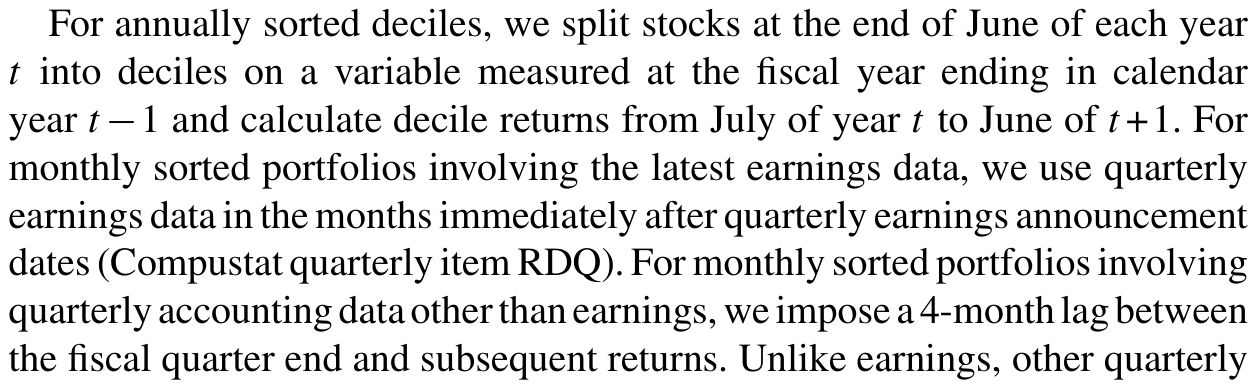
\includegraphics[width=0.78\linewidth,height=0.8\textheight,keepaspectratio]{figures/ref-timing.png}\end{frame}
\begin{frame}{HXZ A.1.1：sue}\centering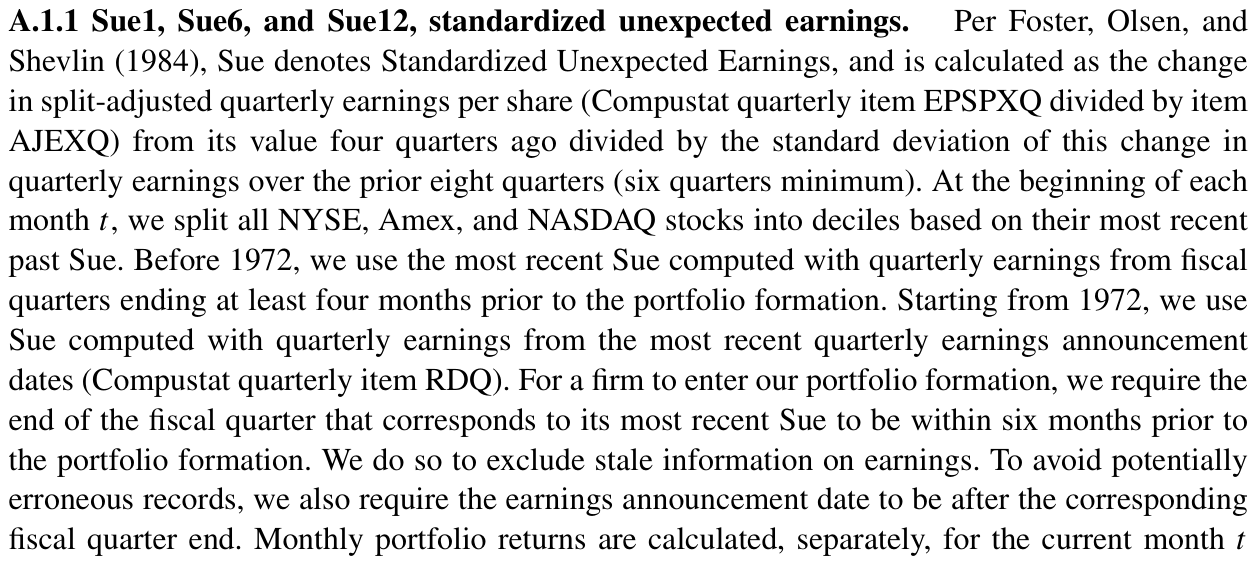
\includegraphics[width=0.78\linewidth,height=0.8\textheight,keepaspectratio]{figures/ref-sue.png}\end{frame}
\begin{frame}{HXZ A.1.2：abr}\centering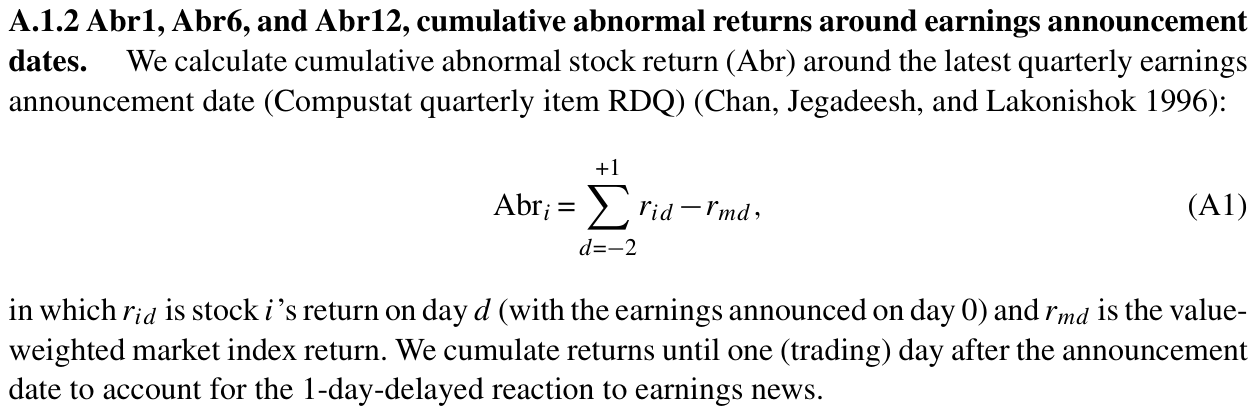
\includegraphics[width=0.78\linewidth,height=0.8\textheight,keepaspectratio]{figures/ref-abr.png}\end{frame}
\begin{frame}{HXZ A.1.3：re}\centering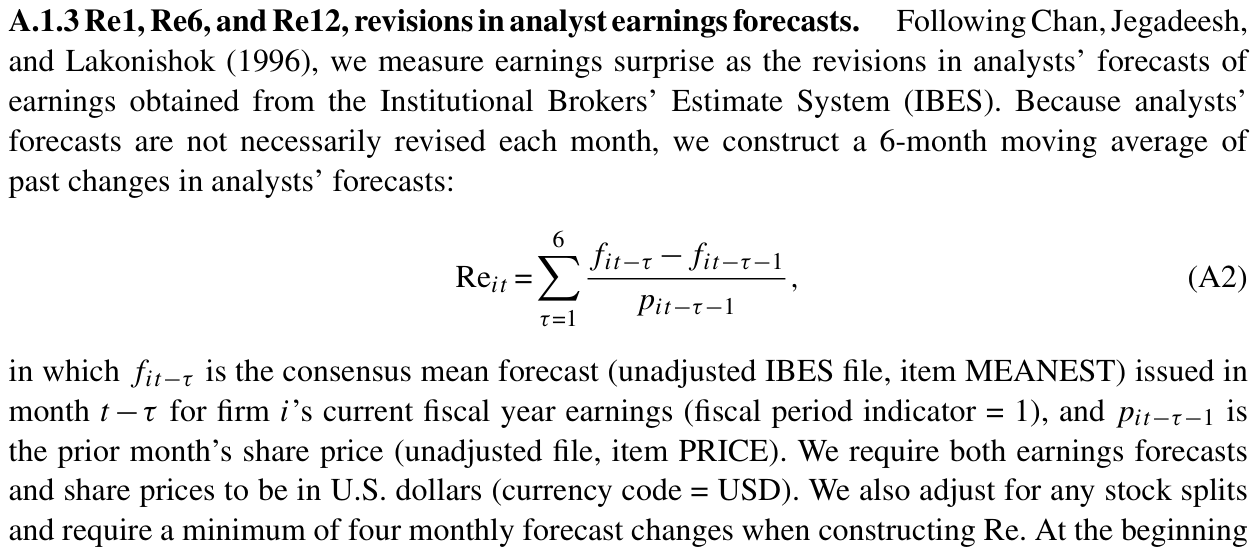
\includegraphics[width=0.78\linewidth,height=0.8\textheight,keepaspectratio]{figures/ref-re.png}\end{frame}
\begin{frame}{HXZ A.3.10：ni}\centering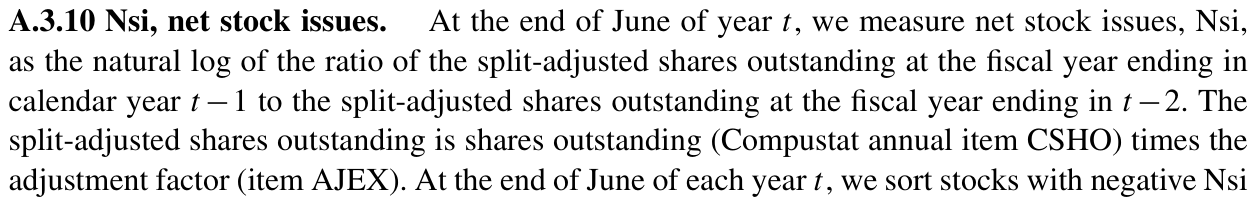
\includegraphics[width=0.78\linewidth,height=0.8\textheight,keepaspectratio]{figures/ref-ni.png}\end{frame}
\begin{frame}{HXZ A.4.3：roa}\centering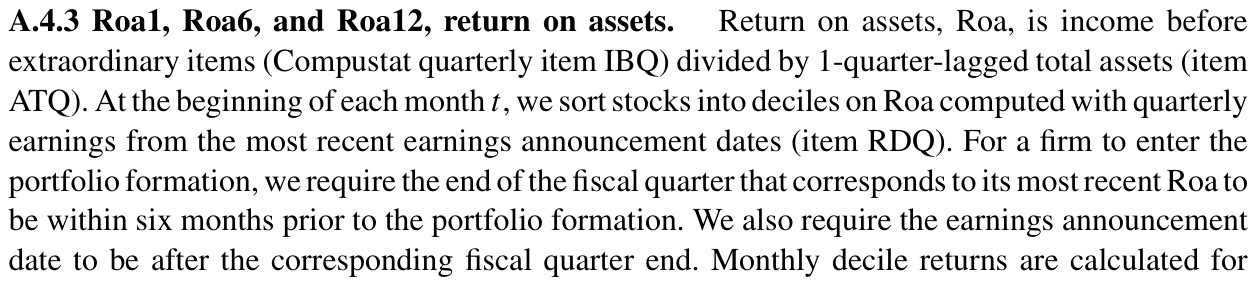
\includegraphics[width=0.78\linewidth,height=0.8\textheight,keepaspectratio]{figures/ref-roa.png}\end{frame}
\begin{frame}{GHZ：cinvest}\centering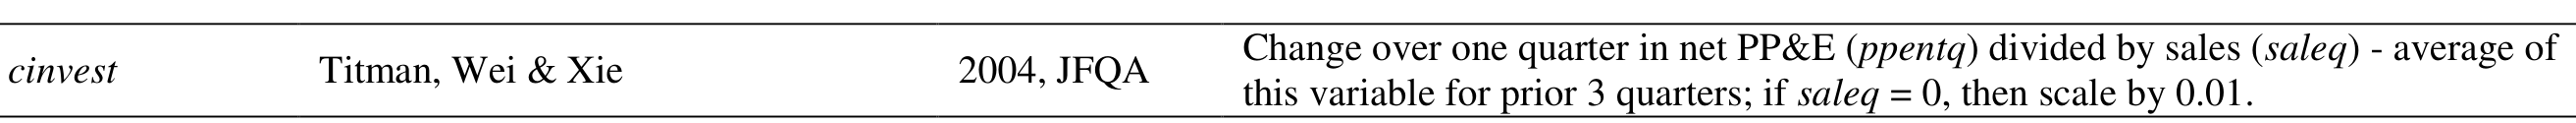
\includegraphics[width=0.78\linewidth,height=0.8\textheight,keepaspectratio]{figures/ref-cinvest.png}\end{frame}

\end{document}
